\chapter{Development of TestBench}
\label{ch:testbenchdevelop}
  
  The estimated time for developing Testbench 4 was from six to eight weeks.
  Our team had four members:
  \begin{itemize}
    \item Anthony Guerreiro - developer.
    \item Dmitrii Rogozin - developer.
    \item Jonatan Kronqvist - tech lead.
    \item Mika Mutajarvi - developer.
    
  \end{itemize}
  
   This is a short period of time and to manage delivering a good quality
   product you have to minimize overhead costs. We believe that a team should choose tools
    and methodology which suits its purposes. 
    Our team decided to use Scrum and Test Driven Development (TDD) for managing
    product development and try to be agile and flexible \cite{scrumSite}. 
    We decided to have two week sprints.

  \section{Scrum}
    Scrum is a management and control process that helps developers to focus on building software 
    that meets business needs. Management and teams are able to get their
    hands around the requirements and technologies and deliver working software,
    incrementally and empirically. The Scrum Team consists of a Product Owner,
    the Development Team, and a Scrum Master.
    
  \textbf{Product Owner} (PO) decides what features should the product have to
  maximally increase the satisfaction of the end user of the product and puts this features to the backlog.
  Backlog is a set of features in priority order.
  
  \textbf{Development team} is
  a set of professionals that are working on implementing features of the product. 
  The team size should be from three to eight people. The team should work only on tasks from the backlog.
  
  \textbf{Scrum master} is a person who should help the team to increase their
  productivity by enhancing the understanding of teams strengths and weaknesses.

  The main idea of scrum is that development is done in short-time periods
  called sprints. Each spring consists of several phases:
  \begin{itemize}
    \item  Sprint planning - when team decides what tasks should be done during the
  sprint.
  \item   Main phase - when actual development is done.
  \item Sprint review - when team shows the results to the product owner.
  \item Retrospective - when team discuss what can be improved.
  \end{itemize}
 
  Sprint may take from one to four weeks. The development team should decide
  what sprint length suits their needs. During sprint planning the team chooses
  which tasks will be moved from a product backlog to a sprint backlog.
  One of the restrictions is that the task in sprint backlog should be done in one sprint.
  If the team thinks that the task can not be finished in one sprint this task
  should be divided into several subtasks. 
  
  Having such one sprint tasks helps the scrum team to keep track of the
  progress easily and gives an opportunity to receive feedback for each
  completed task at the end of the sprint. This helps to detect problems at the early stages, when
  the errors does not have a tremendous impact.
  Even if a feature was misunderstood by the development team
  and the team  has to redone it completely, the team wastes time equal to the
  length of the spring at maximum. While in a classical waterfall model,
   a sequential design process in which progress is seen as flowing steadily through 
   the phases of all development stages, 
  the error might be found much more lately, which will have a bigger negative impact.

  Another feature of Scrum is self organization of the team. The team should
  decide by itself which toolset to use. Tasks in scrum are not assigned to
  developers by a manager, but instead developers take items from the backlog by themselves.
  This approach saves time and reduces stress, because a person can pick a task,
  which he likes and understands. Developers pick tasks that they
  can finish before the end of the sprint.

  In our case we were not developing a new product, but releasing a new version.
  We did not find any arguments to change the tools that were used in the
  previous release we describe them in section \ref{sec:toolsused} .

  \section{Test Driven Development}
  TDD is a very popular methodology of a software development. The main idea is
  to write tests first and then code. The main benefits of such approach are
  the following:
      \begin{itemize}
        \item The developer is sure that his code works as intended, because all
        his code is tested.
        \item The errors are found at early stage of the development cycle, which
        reduces the cost of fixing problems.
      \end{itemize}
      
      Three laws of TDD \cite[pp122]{cleancode}[Book page 122]
        \begin{itemize}
          \item You may not write production code until you have written a failing unit test.
          \item You may not write more of a unit test than is sufficient to fail.
          \item You may not write more production code than is sufficient to pass the currently failing test.
        \end{itemize}
    
  During the project we implemented two different type of tests - unit tests and
  integration tests. 
  
  Unit tests are used for testing individual parts of source
  code, for example a method which parses a regular expression or an utility
  class, for comparing two screenshots.
  
  Integration tests combine several parts of the application and test 
  interaction between them. In our case integration test consist of a Web page
  running as a Vaadin application on a server and a TestBench test class. When
  a TestBench test starts it opens the Web page in the browser and operates on
  the elements on the Web page, by simulating user actions like clicking or typing
  and compare actual and expected behaviour of the elements. 
      
  \section {Tools used}
  \label{sec:toolsused}
  
  \subsection{Maven}
  Maven is a java-based software project management and comprehension tool
  \cite{maven}.
  Maven is based around the central concept of a build life cycle. This means
  that the process for building and distributing a particular project(artifact) is clearly defined.
   There are three built-in life cycles:
  default, clean and site. Users can define their own life cycle. 
  
  Life cycles  consist of phases.  The default life cycle includes the following phases:
  \begin{itemize}
    \item validate - validates the project is correct and all necessary
    information is available.
    \item compile - compiles the source code of the project.
    \item test - tests the compiled source code using a suitable unit testing
    framework. These tests should not require the code be packaged or deployed.
    \item package - takes the compiled code and packages it in its distributable
    format, such as JAR.
    \item integration-test - processes and deploys the package if necessary into
    an environment where integration tests can be run.
    \item verify - runs any checks to verify the package is valid and meets quality criteria
    \item install - installs the package into the local repository, for use as a
      dependency in other projects locally.
    \item  deploy - copies the final package to the remote repository for
    sharing with other developers and projects.
  \end{itemize}
  
  The life cycle phases are executed sequentially. For  example 
  running maven deploy executes all the  previous phases (validate, compile,
  test).
  
  All maven configurations are specified in the Project Object Model (POM) file.
  POM is an XML file that contains information about the project and configuration
   details used by Maven to build the project. 

  Maven reduces the complexity of developing and maintaining big projects.
  Nowadays applications may depend on dozens of third-party libraries and
  frameworks. Managing those dependencies manually is very time consuming. Maven
  finds  and downloads the exact version of the library and adds it to the
  project.
  
   Maven profiles allow to have different configurations of the
  application for development and production or testing. All the maven
  configurations are in the same POM file, that is why editing and sharing
  configurations between members of the team is very easy. 

  Finally, you have a set of predefined configurations for your application
  for the whole team and any developer can checkout POM file from the repository
  call ``mvn deploy'' and he will have the same version of the application with all
  the specified parameters and downloaded dependencies. If you updated
  your dependencies or fixed an error, all your team members
  have to just checkout the new version of a POM file.
 
  \subsection{Trac}
  Trac is an enhanced wiki and issue tracking system for software development
  projects \cite{trac}. Trac may include several projects. Users or developers
  can create tasks (also called tickets) for these projects. 
  
   Before development a new release a product owner goes through 
   the list of the tickets and add them to a new milestone.
  Milestone is a plan for the next release, which includes a set of tickets.

  Tickets have different value for the end user, but developers can not always
  assess that value by themselves. Product owner should help the development team
   to figure out the
  value of each ticket for the end user. Based on the value and time estimation
   each ticket should be prioritized.
  Prioritizing tickets is a very important task and should be done as soon as
  possible, preferable before coding starts. This gives a clear vision for all
  members of the team what should be done.

  In the TestBench 4 project we used the Trac milestone as a product backlog. On
  the sprint planning we estimate which tasks can be completed at the end of the sprint 
  and move them to the sprint backlog. As a sprint backlog we used a scrum
  board.
  
  Scrum board is a white board, divided into several sections for example ``to be done'', ``in progress'', 
  ``in review'',
  ``closed''. Paper stickers represent tickets and the person who is working on
  the ticket.  
  The workflow is the following - a developer picks the
  ticket from the sprint backlog queue called ``to be done'' 
  writes his name on the sticker and move it to the ``in progress'' section.
  After he submitted a patch to the code review he moves the sticker to another
  section and so on.
  
  Looking to the scrum board gives you a brief summary of every team member tasks and 
  also the current sprint progress. One can also find more detailed information
  about tickets and the project progress in Trac.
 
 \subsection{Git}
  As a version control system we used \textbf{Git} - distributed revision control system
  which focuses on speed, data integrity, and support for distributed,
  non-linear workflows \cite{gitDocs}. There are two types of revision control
  systems :
  
   \begin{itemize}
   \item Client-server - such version control systems as SVN and CVS, have a 
    a remote database, which stores the history of files. Systems like CVS,
    Subversion, Perforce, Bazaar store information as  a list of file-based
    changes \cite{gitBasics}. When working with such systems a developer copies
    the latest snapshot of files to a local machine makes changes and then
    pushes his changes to the remote database. All the information about
    files history is available only from the remote database, locally only
    snapshots of files are stored. Almost every SVN command requires a
    connection to the remote database, this brings a network delay for
    SVN commands.
    
   \item Distributed revision control systems such as Git, are structured on a
    peer-to-peer basis: instead of one centralised repository. Every developer
    has his own local repository with the history of all changes. There is no
     main repository as in client-server control systems, all repositories are
     ``equal''. Changes can be sent between any of these repositories, though
     in practise developers create a ``master'' repository,
      where everyone push their own changes and pull
    changes made by other developers.
  \end{itemize}
  
  One of the biggest advantage of Git, that it lets developers to
  have their local history of changes and commits, 
  but when pushing changes to the master repository they can merge these
  changes as one commit.
  This helps on one hand keep a local history of intermediate steps for
  developer, but on the other hand have only commits for completed changes
  or features in the master repository. 
  
  Git has a powerful set of tools including  Unix commands. For example to find
  all commits made by one person you can use log command and pipeline it to a pattern
  matching command like ``grep''.
  
   Git-blame command allows you to see the history of every line of your source
   code. If you have questions about some particular few lines of code,
   you can find an author of those lines and ask him directly.
   
   Git-bisect command - is a binary search against revision graph, which helps to find the commit which
   introduced a bug.

  \subsection{Teamcity}
  Teamcity - is a Web-based build management and continuous integration tool
  \cite{teamcity}.
  Teamcity allows running multiple builds and tests under different platforms and environments.
  Teamcity build combines maven, ant builds, git commands and bash scripts.
  
  Teamcity builds may be started automatically or manually. One option is to create a configuration 
  to run all  tests every night or to setup running tests on every git commit. Teamcity
  provides also build dependencies. If project A depends on a library B,
  Teamcity will first build library B with its dependencies and then start build
  project A.
  
  During the development cycle we used four different configurations.
  \begin{itemize}
  \item Running tests on every git commit. This configuration is started when
  Gerrit \ref{sec:gerrit} patch is submitted.
   Running all tests for all browsers is very time consuming and may take several hours. 
   That is why this configuration includes only JUnit tests and PhantomJS
   \cite{phanotmSite} tests. PhantomJS is a headless browser used for testing Web-based applications.
   Headless browsers does not have GUI and can be controlled via command line
   interface. Running those tests gives a developer a fast feedback, if his changes caused problems.
   
   \item Running all tests on the latest commit every night. This build triggers
   at specific time every night, when servers load is lower than during the day.
    This configuration includes all the heavy tests for specific browsers. All
    the tests are run on Google Chrome, Mozilla Firefox and Internet Explorer 8, 9, 10 and 11. 
    For every test suite Teamcity will run the specific browser on a test
    cluster. Running such tests is very resource consuming, but provides a
    confidence that the application is supported by all browsers.
    
    \item Snapshot build is run every night. This build publishes the latest
    version of the product to a maven repository.  Users can download
    the snapshot build with the latest version of the product, if they want to
    test new features, but do not want to wait for the release build.
    
    \item Release build is run when the team releases a new version of the
    product. This includes building all the dependencies, running all the tests,
    specifying the version of the product, creating release notes, making tag in
    the Git repository, publishing a new version to maven repository and Vaadin
    Web site.
   \end{itemize}

\subsection{Gerrit}
\label{sec:gerrit}
  Gerrit is a Web-based code collaboration tool \cite{gerrit}. Gerrit allows
  developers to review patches made by other developers.
   Gerrit has a very easy system of evaluating patches:
  \begin{itemize}
  \item -2 (veto) - patch has major problems.
  \item -1 (disapprove) - patch has minor problems.
  \item +1 (approve) - no problems found.
  \item +2 (approve) - can be pushed to master.
  \end{itemize}
  
  The difference between +1 and +2 is that the patch can not be pushed to git
  repository without having +2. The reviewer can give +1 if he is not sure about 
  his level of competence  and want someone else to inspect the patch. 
  There are might be several configurations of the review process,
  figure \ref{fig:gerritTestbench} shows the process used in the
  TestBench 4 project.

  Firstly, a developer submits his changes(patch) to Gerrit. Gerrit triggers the
  specific build in Teamcity. This build includes building the project and
  running tests. After this step is finished, Teamcity returns a report about the build,
  if there are problems the report is send to the developer and the patch is marked as -2. If all
  tests pass Gerrit marks the patch as ready for review and put it to the list
  of waiting for review patches.
  Afterwards the reviewer evaluates the patch. Given the patch -1 or -2 means
  that the developer should fix the problems, and submit the next version of the patch. 
  The process continues until the patch is marked as +2,
    meaning in can be pushed to git master repository.
    \begin{figure}
    \centering
      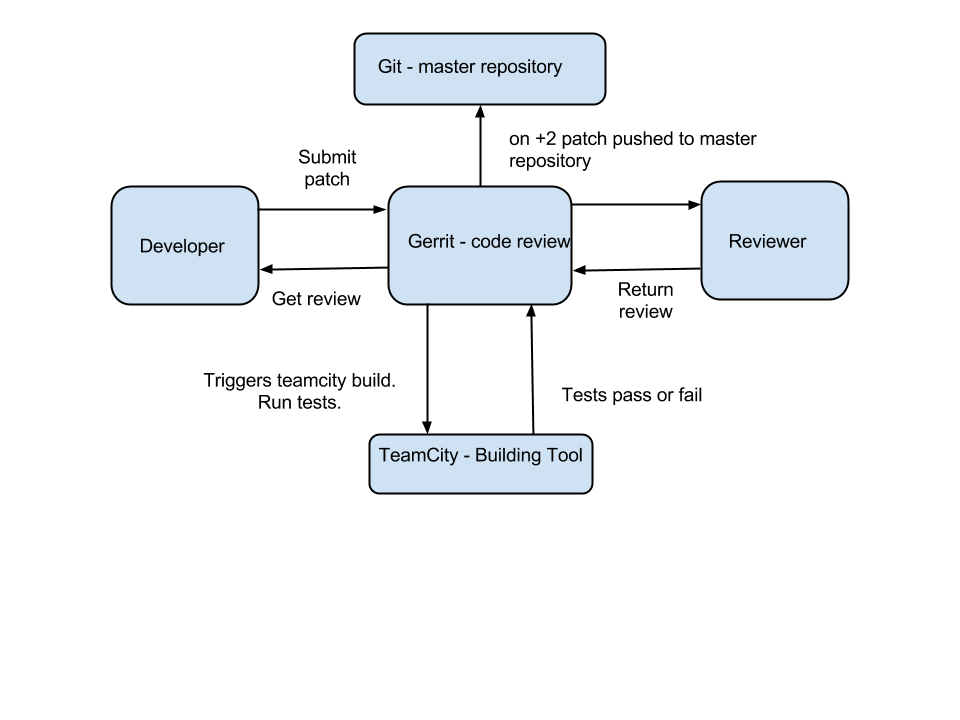
\includegraphics[width=0.75\textwidth]{gerrit1.png}
      \caption{Gerrit structure}
      \label{fig:gerritTestbench}
    \end{figure}
    
  Code review helps team members to follow similar code conventions, 
  keep code clean and find bugs. Also code review helps developers to know more about 
  the whole project they are working in. Integrating Gerrit with an automated build tool, 
  such as TeamCity, allows to run tests before publishing commit for review. 
  The patch with failing tests is rejected automatically and an email with report
   for all failing tests sent to the author of the patch. 
   As an overall code review helps to keep source code quality on a higher level.

  \section{Architecture design}
   
   We have divided TestBench into two modules: TestBench core and TestBench API. Having
two modules and two separate build configurations for them, allows to build only
API module and keep core module as it is. Core module includes fundamental features,
 like client-server communication, finding
elements on a Web page and test parallel execution. API module includes
classes and methods for simulating Vaadin components features, like clicking a
Vaadin button or navigating in a Vaadin menu component. TestBench core
module is steady and should not be changed frequently. TestBench API
module, on the contrary, would change often, because of adding new API.

Testbench-apimodule version number matches the compatible Vaadin framework version.
As a development team we think that having matching Testbench-api and framework versions will help to solve
 compatibility issues, showing the users which TestBench and framework versions they have to use. 
   
 TestBench is written in Java and uses inheritance for code reuse and
  extensibility. The hierarchy of classes in TestBench consists of many tens of
  classes and each class has tens of methods.
  Here we will describe the most important classes and the basic principles as
  shown in Figure \ref{fig:classdiagram}.
	\begin{figure}
	\centering	
	    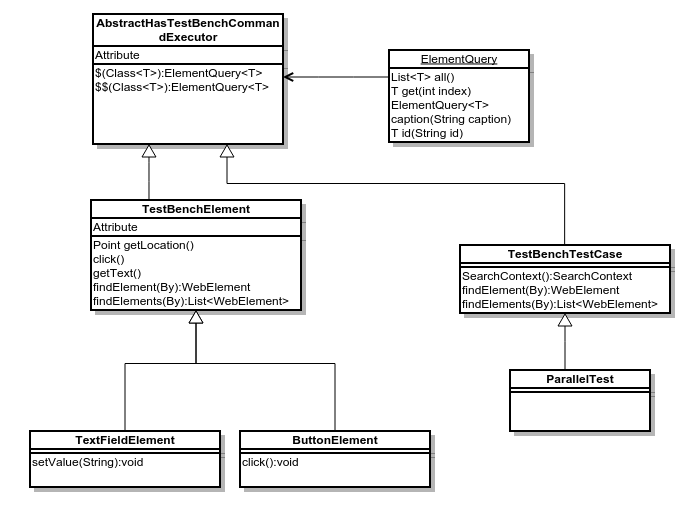
\includegraphics[width=0.75\textwidth] {umlDiagram.png}
	    \caption{Testbench class diagram}
	    \label{fig:classdiagram}
  \end{figure}

\textbf{TestBenchCommandExecutor} handles client server communication
and provides screenshot comparison implementation.

\textbf{AbstractHasTestBenchCommandExecutor} class provides  `\$(Class clazz)'
and `\$\$(Class clazz)' methods which create a query for searching elements of
the given type.
 `\$' method builds a recursive search query and `\$\$' a non-recursive one.
 Non-recursive search query looks only for direct children of the element, while
 it is recursive analog looks through all children of the element. Children
 elements are inner HTML elements. In example \ref{lst:domexample}
   button and check box input elements are children elements of the div element
   with id id1.
 \lstset{style=console}
\begin{lstlisting} [caption=Simple DOM example,label={lst:domexample}]
<div id="id1">
	<input type="button">
	<input type ="checkbox">
</div>
\end{lstlisting}
  
  
\textbf{ElementQuery<T>} used for locating Web elements, such as Vaadin buttons,
text fields, labels  on a Web page.
Generic parameter T specifies the type of a searched element.
 ElementQuery class provides methods for searching the element based on
 elements id, class, caption or other criteria. These methods can be considered
 as filters in the query. ElementQuery uses the builder pattern, 
 which helps to add several filters to build a specific query and after
 the query is built execute it.

Example \ref{lst:searchButtons} shows finding all children elements of the
parent element  which are buttons:
  \lstset{style=a1listing}
\begin{lstlisting} [caption=Search for all buttons,label={lst:searchButtons}]
AbstractHasTestBenchCommandExecutor elem = getParentElement();
List<Button> allButtons=elem.$(ButtonElement.class).all();
\end{lstlisting}
  
To restrict search for buttons with caption ``ok'' we add a caption filter to
the query see example \ref{lst:searchOkButtons}.
  \lstset{style=a1listing}
  \begin{lstlisting} [caption=Search for for button  with caption "ok", label={lst:searchOkButtons}]
AbstractHasTestBenchCommandExecutor elem =  getParentElement();
List<Button> allButtons=elem.$(ButtonElement.class)
	.caption("ok").all();
  \end{lstlisting}
  
\textbf{TestBenchElemenet} - is a base class for operating on Vaadin components.
It includes methods to access properties common to all Vaadin elements,
such as getSize, getLocation, getCssValue, etc.
TestbenchElement class uses Selenium WebElement class as a foundation and extend
its functionality by using JavascriptExecutor,
which allows to execute JavaScript code, and change the default element behaviour.

\textbf{TestBenchTestCase} - an abstract super class of a TestBench test.

\textbf{ParallelTest} - supports running test in parallel threads with several
browser configurations see \ref{sec:paralelTesting} for more details.

\textbf{ButtonElement, MenuBarElement, TableElement}, etc. - implement specific
Vaadin class features. The default naming conventions is Vaadin component name
plus ``Element''. In other words ButtonElement accesses buttons methods,
TableElement table methods and so on.

The important aspect is that hierarchy of TestBench elements is similar to
Vaadin elements.
That gives more flexibility when writing tests. The  developer can
specify concrete class for getting access to specific methods of the element see example \ref{lst:specificExample}.
 
\lstset{style=a1listing}
\begin{lstlisting} [caption=Test for Vaadin table, label={lst:specificExample}]
  TableElement table= getElement();.$(TableElement.class).first();
  TableRowElement row=table.getRow(0);
 \end{lstlisting}
 
or use a more generic class to utilize method of a parent class, for example get
caption of all elements, see example \ref{lst:genericExample}.

\lstset{style=a1listing}
\begin{lstlisting} [caption=Caption test for Vaadin elements, label={lst:genericExample}]
List<TestBenchElement> elements=
	getElement().$(TestBenchElement.class).all();
List<String captions=new ArrayList<String ();
for(int i=0;i<elements.size();i++) {
	captions.add(elements.get(i).getCaption());
}
\end{lstlisting}

\section {Basic test case structure}
To use TestBench, the test case class should extend the TestBenchTestCase class,
which provides the WebDriver and ElementQuery APIs. A developer
can configure TestBench test by using following annotations:
\begin{itemize}
  \item @Rule -defines certain TestBench parameters.
  \item @Before - the annotated method is executed before each test.
  \item @Test - annotates the tested method.
  \item @After - the annotated method is executed after test.
\end{itemize}

A typical test case structure is the is the following:
\begin{itemize}
  \item Set TestBench parameters.
  \item Open the tested Web page URL.
  \item Find an element for interaction (Button, TextField).
  \item Interact with the elements (click buttons,menus,etc.).
  \item Find an element to check.
  \item Get and the value of the checked element.
  \item (optional) get screenshot.
\end{itemize}

A complete example of test UI class \ref{lst:appTestUI}  and a TestBench test
class \ref{lst:appTestClass} can be found in appendix A \ref{appendixA}.

\section {Results}
During the TestBench 4 development our team added new API to ease writing tests
for Vaadin applications. We added helper methods for MenuBarElement,
TreeTableElement, TwinColSelectElement,PopupDateFieldElement etc. Besides a
ParallelTest class was introduced, which supports running tests concurrently in
several threads. Overall we have completed 41 ticket
and the detailed information about these tickets can be found in table \ref{table:tickets} in appendix B \ref{appendixB}.

To improve User Experience (UX) we have tried to reduce an amount of
configuration needed for using TestBench. We provide a simple test as a
part of a build-in configuration.
Developers can use it as an example and extend it for their own requirements. Users may create a sample
Vaadin application via GUI using Vaadin Eclipse plugin or Maven build tool.

Vaadin Eclipse plugin provides a wizard for creating a new Vaadin application.
The wizard suggest default values for project settings, which user can change or just fill
the project name and use default values for project folder structure, theme
name, deploy configuration, etc \ref{fig:vaadinPlugin}. After finishing the
wizard setup Vaadin plugin creates a Vaadin project which can be
deployed and run on a Web server. Vaadin plugin also adds a simple button click
TestBench test to the project which can be run as a JUnit test.
  \begin{figure}
  \centering
  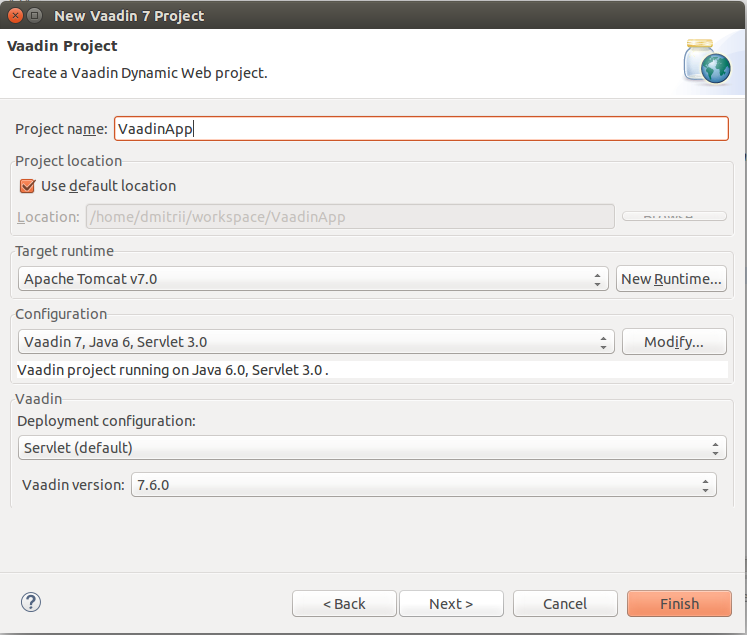
\includegraphics[width=0.75\textwidth]{vaadinPlugin}
  \caption{Vaadin project wizard}
  \label{fig:vaadinPlugin}
  \end{figure}

To create a sample Test via Maven user should use a Vaadin Maven
archetype see \ref{lst:mavenexample}.
\lstset{style=console}
\begin{lstlisting}[caption=Create Vaadin sample application command.,label={lst:mavenexample}]
mvn archetype:generate 
	-DarchetypeGroupId=com.vaadin
	-DarchetypeArtifactId=vaadin-archetype-application
	-DarchetypeVersion=LATEST
\end{lstlisting}

After beta release we made several usability tests.
A Vaadin developer, without experience in using TestBench, manages to create and 
run a simple ``button-click'' test in less that 15 minutes. 

Vaadin TestBench 4 is released with Commercial Vaadin Add-On License 
(CVAL). But if you want to look results of our work and try it out you have two
options:
\begin{itemize}
  \item Free 30-days trial period.
  \item One year non-commercial license. All the details how to get it are at
  Vaadin blog \cite{vaadinBlog}.
\end{itemize}

Vaadin framework is using TestBench as a main testing tool for acceptance
testing. Overall Vaadin framework has about six thousand TestBench tests which
are run nightly and also before every Vaadin release.
